%%%%%%%%%%%%%%%%%%%%%%%%%%%%%%%%%%%%%%%%%
% Twenty Seconds Resume/CV
% LaTeX Template
% Version 1.1 (8/1/17)
%
% This template has been downloaded from:
% http://www.LaTeXTemplates.com
%
% Original author:
% Carmine Spagnuolo (cspagnuolo@unisa.it) with major modifications by 
% Vel (vel@LaTeXTemplates.com)
%
% License:
% The MIT License (see included LICENSE file)
%
%%%%%%%%%%%%%%%%%%%%%%%%%%%%%%%%%%%%%%%%%

%----------------------------------------------------------------------------------------
%	PACKAGES AND OTHER DOCUMENT CONFIGURATIONS
%----------------------------------------------------------------------------------------
\documentclass[letterpaper]{twentysecondcv} % a4paper for A4
\usepackage[utf8x]{inputenc} % Включаем поддержку UTF8  
\usepackage[russian]{babel}  % Включаем пакет для поддержки русского языка 
%----------------------------------------------------------------------------------------
%	 PERSONAL INFORMATION
%----------------------------------------------------------------------------------------

% If you don't need one or more of the below, just remove the content leaving the command, e.g. \cvnumberphone{}
\profilepic{111111.jpg} % Profile picture

%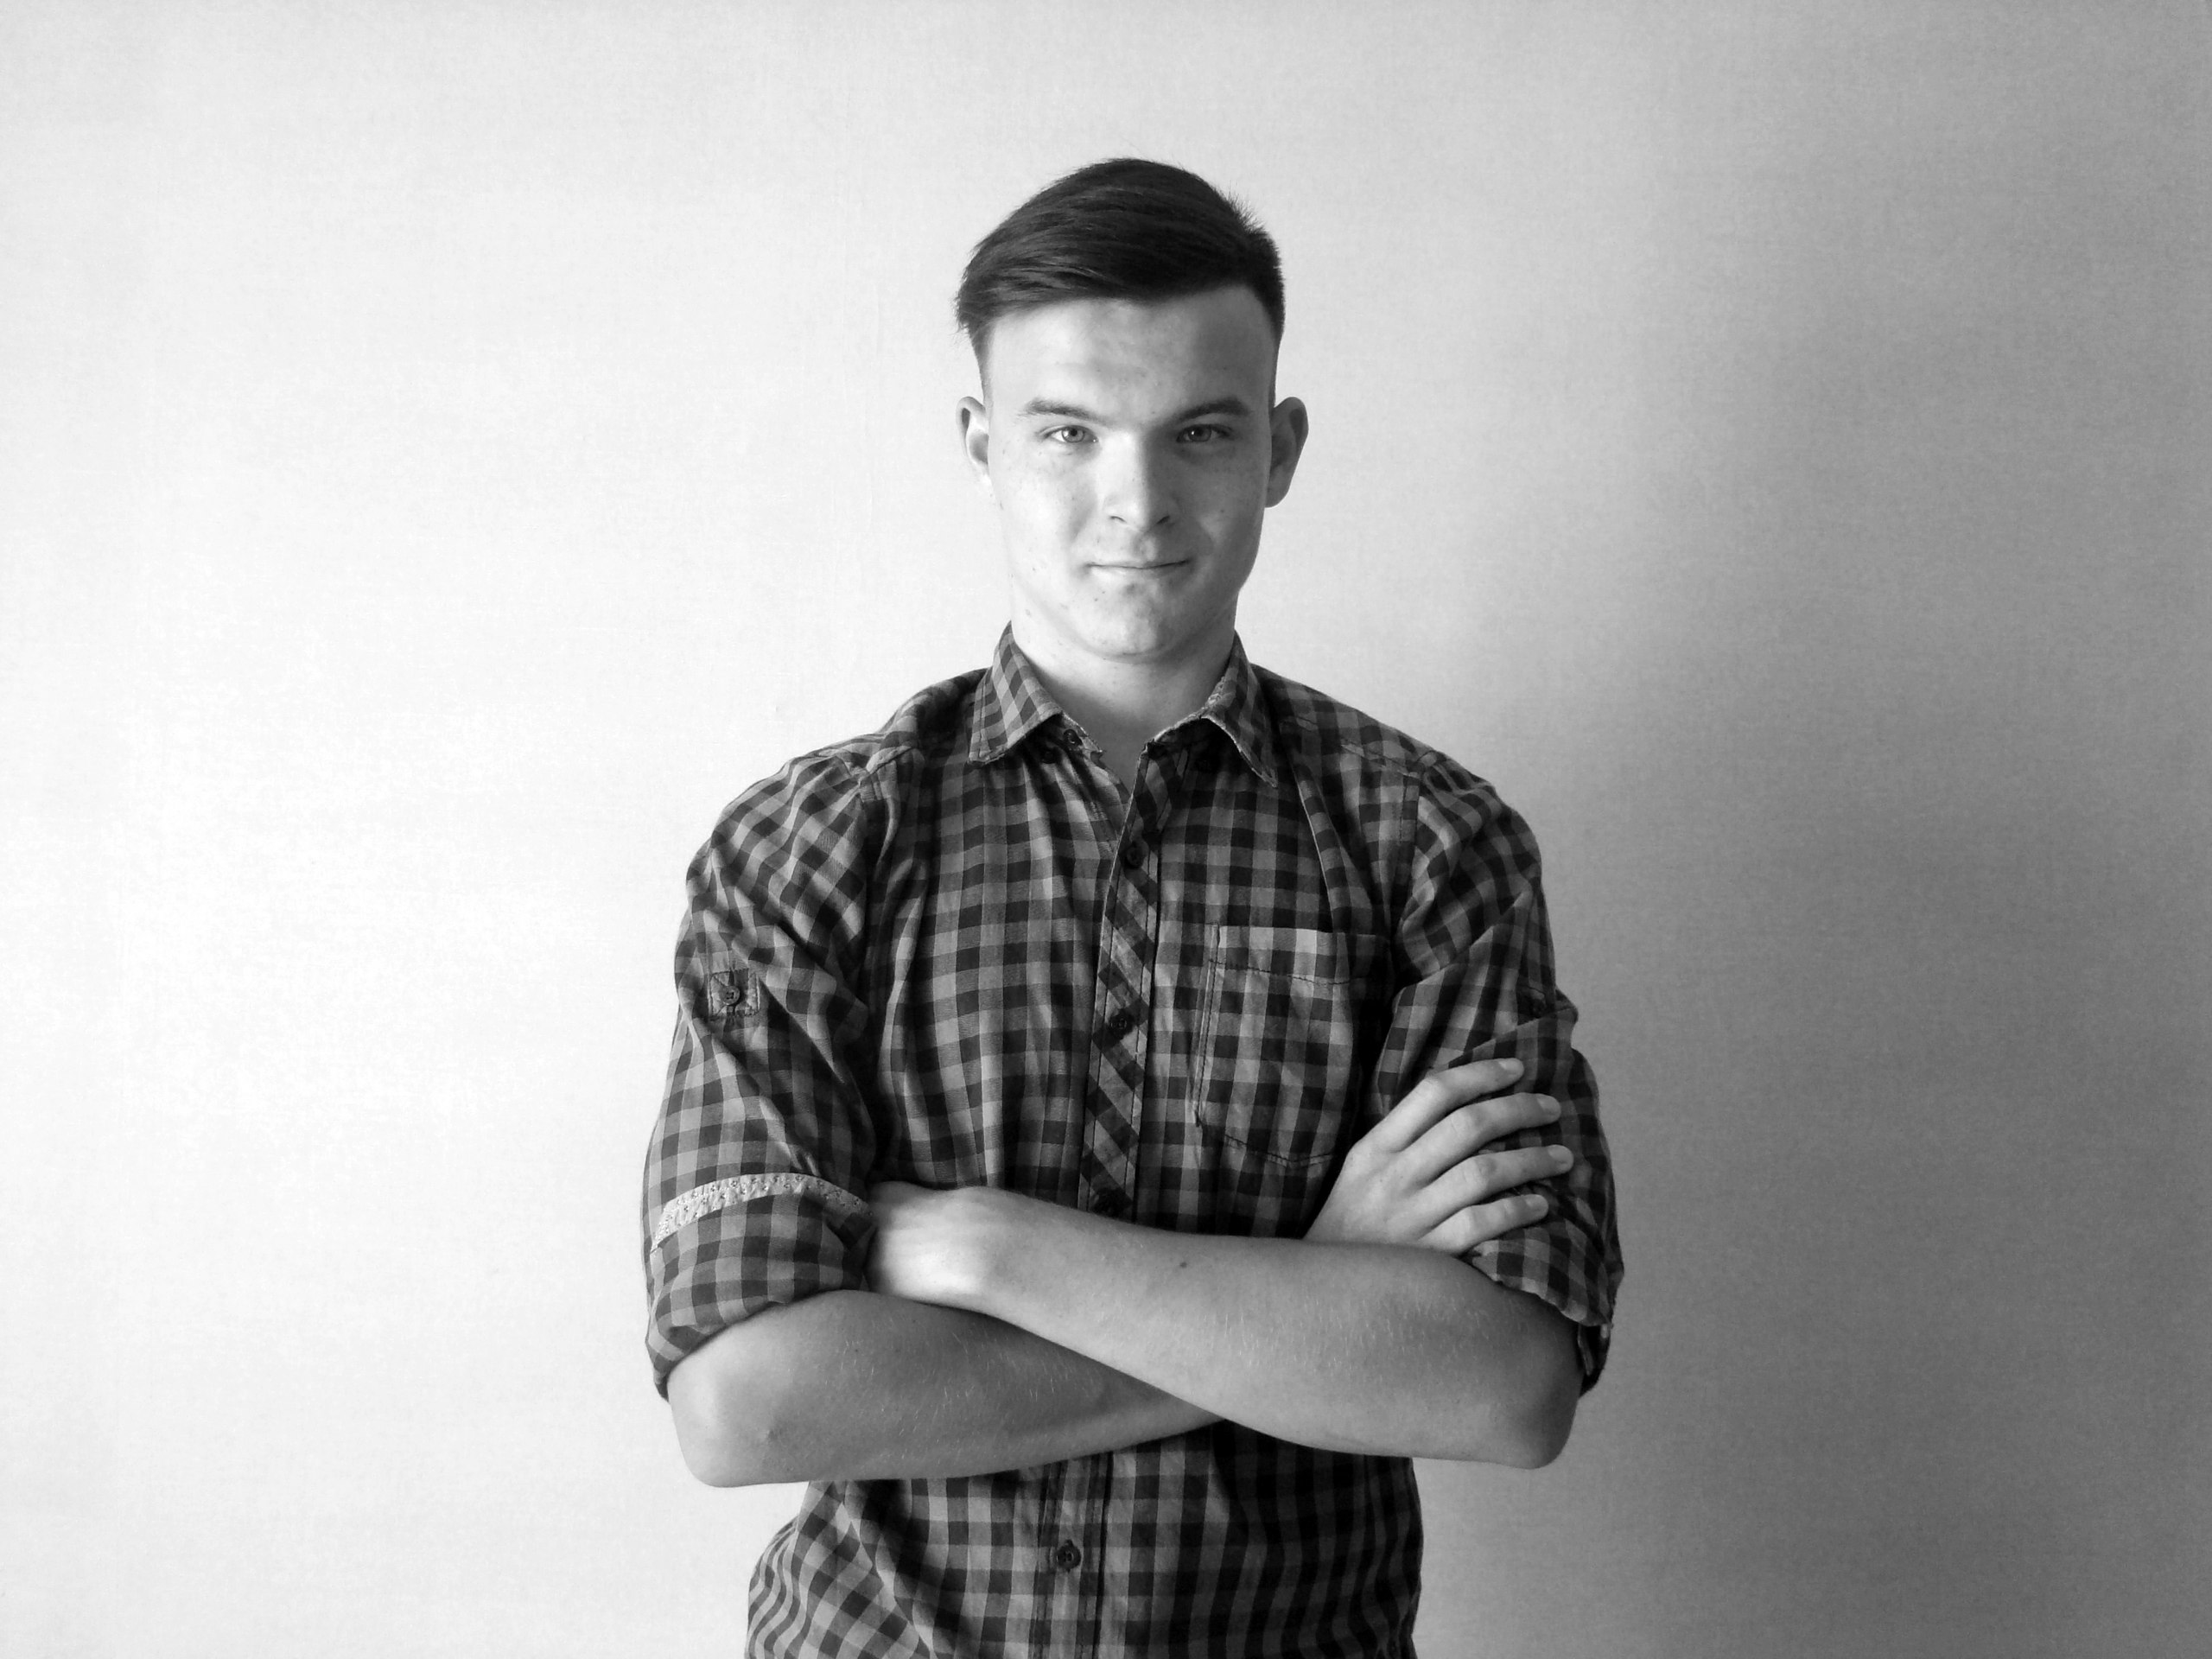
\includegraphics[scale=0.18]{1.jpg}

\cvname{Кирилл Недостоев} % Your name
\cvjobtitle{} % Job title/career

\cvdate{7 октября 1998} % Date of birth
\cvaddress{Москва, Россия} % Short address/location, use \newline if more than 1 line is required
\cvnumberphone{+7 915 030 96 11} % Phone number
\cvsite{\href{https://github.com/inedostoev}{https://github.com/inedostoev}} % Personal website
\cvmail{nedostoev.ka@phystech.edu} % Email address

%----------------------------------------------------------------------------------------

\begin{document}

%----------------------------------------------------------------------------------------
%	 ABOUT ME
%----------------------------------------------------------------------------------------

\aboutme{} % To have no About Me section, just remove all the text and leave \aboutme{}

%----------------------------------------------------------------------------------------
%	 SKILLS
%----------------------------------------------------------------------------------------

% Skill bar section, each skill must have a value between 0 an 6 (float)

\skills{{Рабоспособность/5.5},{Golang/3}, {Win API/3},{git/4},{Linux/4},{Python/4},{{C/C++}/5}}
%------------------------------------------------

 %Skill text section, each skill must have a value between 0 an 6
%\skillstext{{lovely/4},{narcissistic/3}}


%----------------------------------------------------------------------------------------

\makeprofile % Print the sidebar

%----------------------------------------------------------------------------------------
%	 INTERESTS
%----------------------------------------------------------------------------------------

%\section{Interests}

%The heroine and the dreamer of Wonderland; Alice is the principal character.

%----------------------------------------------------------------------------------------
%	 EDUCATION
%----------------------------------------------------------------------------------------

\section{Образование}

\begin{twenty} % Environment for a list with descriptions
	\twentyitem{2016 - 2020}{Бакалавриат}
	{\newline Московский физико-технический институт}
	{\newline Математика (включая линейную алгебру, теорию вероятностей, дифференциальные уравнения и дискретный анализ)
\newline Общая и теоретическая физика
\newline Программирование (C, C++, Python, assembler)
\newline Предметы базовой кафедры: Многопоточное программирование, архитектура современных микропроцессоров, производительность современных файловых систем, системное программирование 
\newline
\newline Средний балл: 4.64/5.00}

\end{twenty}

\section{Навыки} 

{\textbf{Programming:}} {C/C++, python, assembler, Golang.}\\ 
{\textbf{Operating system:}} Linux, Windows. \\
{\textbf{Extra:}} git, bash, latex. \\
{\textbf{English:}} upper-intermediate. \\

\section{Опыт работы}

\begin{twenty} % Environment for a list with descriptions
	\twentyitem{c марта 2019}{in Acronis Storage - intern}
	
{
\newline 1. Инкрементальный пересчет кодов Рида-Соломона; 
\newline 2. Сбор расширенной статистики с узлов кластера и представление этой статистики в виде heatmap.
\newline 3. Создание асинхронного репликатора изменений файловой системы NTFS (бакалаврская работа)

}
\end{twenty}


\section{Дополнительные техкурсы и проекты}

\underline{\href{https://github.com/inedostoev/Ilab-Technotrack}{Лабораторные работы}} в рамках курса языка C/С++ \\
(МФТИ ФРТК, открытый курс Ilab и Mail.Технотрек, преп. И.Р. Дединский)
        \begin{enumerate}
            \item {Сортировка текстов («Евгений Онегин») [\underline{\href{https://github.com/inedostoev/Ilab-Technotrack/tree/master/Technotrack/Sort}{github}}]
            }
            
            \item Экспертная система – двоичный справочник («Акинатор») [\underline{\href{https://github.com/inedostoev/Ilab-Technotrack/tree/master/Technotrack/MIPTakinator}{ github }}]
            
            \item Символьное дифференцирование выражений («Дифференциатор») [\underline{\href{https://github.com/inedostoev/Ilab-Technotrack/tree/master/Technotrack/diff}{github}}]
            
            \item  Эмулятор CPU («Процессор») [\underline{\href{https://github.com/inedostoev/Ilab-Technotrack/tree/master/Technotrack/CPU}{github}}]
            \begin{enumerate}
                a) Soft-CPU с собственным набором команд \\ b) ассемблер для soft-CPU
            \end{enumerate}
        \end{enumerate}
        
Годовой курс по микроархитектуре от Intel \\
(МФТИ ФРТК, 2 курс)
\begin{enumerate}
    \item Разработка потактового симулятора процессора в команде [\underline{\href{https://github.com/MIPT-ILab/mipt-mips}{mipt-mips}}]
    
    \item Скрипт, предотвращающий commit и push кода с неправильным стилем кода [\underline{\href{https://github.com/inedostoev/codeguidelines}{github}}].
\end{enumerate}

Лабораторные работы в рамках курса по архитектуре STM32 \\
(МФТИ ФРТК, преп. Э. Казиахмедов)
\begin{itemize}
    \item Проект по созданию часов с настраиваемым будильником [\underline{\href{https://github.com/inedostoev/STM32f0_ARM/tree/master/TemplateProject}{github}}]
\end{itemize}

Лабораторные работы в рамках изучения предметов на базовой кафедре \\
(МФТИ ФРТК, Кафедра теоретической и прикладной информатики)
\begin{enumerate}
    \item Многопоточное программирование (преп. С. Бабичев): skiplist, treadpool, fast matrix multiplication. [\underline{\href{https://github.com/inedostoev/ParProg}{github}}]
    
    \item Производительность современных файловых систем (преп. А. Анисимов): utf-8 converter and decoder, ps and lsof utils, B-tree. [\underline{\href{https://github.com/inedostoev/filesystem}{github}}]
    
    \item Архитектура современныз микропроцессоров (преп. А. Костюшко): Лабораторные работы на MS DOS. [\underline{\href{https://github.com/inedostoev/dos-labs}{github}}]
\end{enumerate}
        


\section{Достижения}

\begin{itemize}
    \item Публикация: Программная реализация физически неклонируемых функций, Труды МФТИ Том 12, №2 (46) (2020), 55-63 стр.  [\underline{\href{https://mipt.ru/upload/medialibrary/1ee/5_martvel_55_63.pdf}{ссылка}}]
    \item \textbg{Хакатон:} Phystech.Genesis - Второе место. Работа связана с 3D моделями
\end{itemize}

\section{Личные качества} 

\newline Аналитические способности, работоспособность, коммуникабельность, умение работать в команде, ораторские качества

\section{Внеучебная деятельность} 

\newline Плавание, председатель студсовета ФРТК, организатор Дней Физика в
МФТИ.

%----------------------------------------------------------------------------------------
%	 PUBLICATIONS
%----------------------------------------------------------------------------------------

%\section{Publications}

%\begin{twenty} % Environment for a short list with no descriptions
%	\twentyitem{2018}{ \href{http://itas2018.iitp.ru/media/papers/1570482895.pdf}{Heteroscedastic Gaussian processes and their application to Bayesian optimization}}{\newline Information technologies and systems (ITaS) 2018}

	%\twentyitemshort{<dates>}{<title/description>}
%\end{twenty}

%----------------------------------------------------------------------------------------
%	 AWARDS
%----------------------------------------------------------------------------------------

%\section{Awards}

%\begin{twentyshort} % Environment for a short list with no descriptions
%	\twentyitemshort{2017}{Scholarship of Abramov and Frolov  fund for excellent educational results }


%\end{twentyshort}

%----------------------------------------------------------------------------------------
%	 EXPERIENCE
%----------------------------------------------------------------------------------------

%\section{Experience}

%\begin{twenty} % Environment for a list with descriptions
%	\twentyitem{2017}{Ivannikov Institute for System Programming of the RAS}{\newline laboratory assistant}{Work was associated with compilers and virtual machines, language - C ++}
%	\twentyitem{2018}{Skolkovo Institute of Science and Technology}{\newline Summer internship}{Bayesian optimization research, work with Gaussian processes, improvement of optimization work accuracy}
	
	%\twentyitem{<dates>}{<title>}{<location>}{<description>}
%\end{twenty}



%\section{Skills} 

%{\textbf{Programming:}} {python, C++, matlab, C.}\\ 
%{\textbf{ML:}} sklearn, xgboost, lightgbm. \\
%{\textbf{Data workflow:}} numpy, pandas. \\
%{\textbf{Deep learning:}} pytorch. \\
%{\textbf{Extra:}} bash, latex, git. \\

%\section{MOOCs} 
%\newline  Advanced Machine Learning
%\newline Mathematics and
%Python for data
%analysis at Coursera
%\newline Python at Stepic and
%Coursera 


%\section{Extra courses}

%\textbf{Intel research student laboratory (iLab):}
%\newline C programming language, algorithms and data structures 
%\newline C++ programming language


%\section{Activities}

%\textbf{Mail.ru group student laboratory Computer Science:} 
%\newline teaching assistant for the first year students

%\textbf{Hackathons:} 
%\newline Phystech.Genesis - 2st place. Work with 3d graphics.


%\section{Hobbies and Interests}

%sports (athletic gymnastics, boxing)

% \newline organization of institute
%olympiads, conferences and other
%events


\end{document} 
